\documentclass[sigconf,review]{acmart}

\usepackage{tikz}
\usetikzlibrary{positioning,arrows.meta,fit,backgrounds,calc}
\definecolor{cData}{RGB}{219,234,254}\definecolor{cDataB}{RGB}{37,99,235}
\definecolor{cFeat}{RGB}{220,252,231}\definecolor{cFeatB}{RGB}{22,163,74}
\definecolor{cModel}{RGB}{255,237,213}\definecolor{cModelB}{RGB}{234,88,12}
\definecolor{cEval}{RGB}{237,233,254}\definecolor{cEvalB}{RGB}{124,58,237}

\setlength{\textfloatsep}{7pt plus 2pt minus 2pt}
\setlength{\floatsep}{5pt plus 2pt minus 2pt}
\setlength{\intextsep}{6pt plus 2pt minus 2pt}
\setlength{\abovecaptionskip}{4pt}
\setlength{\belowcaptionskip}{2pt}
\setlength{\abovedisplayskip}{5pt plus 2pt minus 2pt}
\setlength{\belowdisplayskip}{5pt plus 2pt minus 2pt}
\setlength{\abovedisplayshortskip}{3pt plus 2pt minus 2pt}
\setlength{\belowdisplayshortskip}{3pt plus 2pt minus 2pt}

\AtBeginDocument{%
  \providecommand\BibTeX{{Bib\TeX}}}

\setcopyright{none}
\copyrightyear{2026}
\acmYear{2026}
\acmDOI{}
\acmConference[ICAIF '26]{ACM International Conference on AI in Finance}{November 14--17, 2026}{Milan, Italy}
\acmISBN{}

%% ============================================================================
%% v3 -- full reposition for ICAIF '26 (deadline 2026-08-02 AoE).
%% Every number in this file is backed by a committed artifact
%% (TP2MVTransformer/tables/action_list/*, tables/*.json) or by the v2_1 text
%% it revises. Slots that await the collaborator rerun of
%% 67_mlp5_selectivity_and_dsr_fix.py are marked "TODO-RERUN[67]".
%% ============================================================================

\begin{document}

\title{Machine-Learned Conditional Trading of TP2 Violations in SPY American Call Options}
\subtitle{From Near-Arbitrage Theory to Cost-Aware Selection, with a Caution on Comparing Trading Models}

\author{Pawel Polak}
\affiliation{%
  \institution{Stony Brook University}
  \city{Stony Brook}
  \state{New York}
  \country{USA}}
\email{pawel.polak@stonybrook.edu}

\author{Jyotir Manishkumar Patel}
\affiliation{%
  \institution{Stony Brook University}
  \city{Stony Brook}
  \state{New York}
  \country{USA}}
\email{jyotirmanishku.patel@stonybrook.edu}

\author{Omkar Lashkare}
\affiliation{%
  \institution{Stony Brook University}
  \city{Stony Brook}
  \state{New York}
  \country{USA}}
\email{omkarvilas.lashkare@stonybrook.edu}

\renewcommand{\shortauthors}{Polak, Patel, Lashkare}

\begin{abstract}
Call prices are totally positive of order two (TP2) when the ratio of a higher-strike call to a lower-strike call increases with maturity. This property is stronger than the absence of calendar-spread arbitrage. On SPX index options, TP2 violations are rare, revert fast, and are profitable to trade at mid-prices, with hit rates near 100\% per violation. We study the same structure where the theory's proof conditions do not apply: SPY \emph{American} calls, which have early exercise, discrete dividends, and physical settlement. We detect violations in bid/ask quotes and price every trade with spread and commission costs. The near-arbitrage behavior disappears. Trading all 250{,}004 forward-adjusted T1/K2 violation trades over 2021--2026 \emph{loses} \$12.52M (win rate 12.9\%, Sharpe $-1.01$). The signal is only tradable conditionally, and machine learning recovers it. LightGBM, an MLP, a TP2-specific transformer, and an $L_2$-regularized logistic regression each produce positive out-of-sample returns. All are evaluated under the same causal $p\ge0.5$ selection rule. The result holds on rolling walk-forward splits, under $1.5\times$ spread slippage, and under capital-constrained sizing.

Comparing the learned models exposes a methodological problem. Trades are selected by thresholding a recalibrated probability, so ensembling changes each model's trade count ($+75\%$ for the MLP, $-13\%$ for the transformer) and can reverse Sharpe rankings. We call this the operating-point confound. We separate it from model-specific operating-point effects using matched-selectivity curves and seed-dispersion intervals. Under these controls no architecture wins. The feature construction carries the signal.
\end{abstract}

\begin{CCSXML}
<ccs2012>
 <concept>
  <concept_id>10010147.10010257.10010258.10010259</concept_id>
  <concept_desc>Computing methodologies~Machine learning</concept_desc>
  <concept_significance>500</concept_significance>
 </concept>
 <concept>
  <concept_id>10010405.10010481.10010485</concept_id>
  <concept_desc>Applied computing~Economics</concept_desc>
  <concept_significance>300</concept_significance>
 </concept>
</ccs2012>
\end{CCSXML}

\ccsdesc[500]{Computing methodologies~Machine learning}
\ccsdesc[300]{Applied computing~Economics}

\keywords{options trading, total positivity, American options, statistical arbitrage, machine learning, backtest validation, model selection}

\maketitle

\section{Introduction}
\label{sec:intro}

Call prices in the Black--Scholes model, viewed as functions of strike and maturity, are totally positive of order two (TP2). This means the ratio of a higher-strike call to a lower-strike call increases with time to expiry, after adjusting for dividends and interest~\cite{glasserman2026tp2theory}. TP2 is stronger than the absence of calendar-spread arbitrage, and it holds in many, though not all, standard arbitrage-free models~\cite{glasserman2026tp2theory,glasserman2023convexity}. On SPX index options, TP2 violations are rare and usually reverse within a day. They behave as \emph{near-arbitrage} opportunities: strategies that buy the undervalued side of a violating price rectangle and short the overvalued side win 95--100\% of the time at mid-prices, and they beat the index in almost every year of 2000--2022~\cite{glasserman2025tp2}.

This paper asks what remains of that structure where the theory's proof conditions do not apply, and how much machine learning can recover. SPY options are \emph{American-style}, written on a dividend-paying ETF, and settled by delivery of shares. Early exercise, discrete dividends, and assignment risk all fall outside the European, cash-settled setting in which the TP2 theorems are proved~\cite{glasserman2026tp2theory,cosma2020earlyexercise}. We therefore treat TP2 as a hypothesis to test on SPY prices, not as an established property. We detect violations of the forward-adjusted TP2 inequality in bid/ask quotes rather than mid-prices, and we charge every trade the full spread at entry plus commissions. The near-arbitrage behavior does not survive. Trading every detected T1/K2 violation over the 2021--2026 test years---250{,}004 episode-strategy pairs---\emph{loses} \$12.52M under a \$1{,}000-per-trade convention, with a 12.9\% win rate and Sharpe $-1.01$. The SPX study wins 95--100\% of the time at mid-prices; here the same structure loses money. Detecting a violation is not the same as selecting a trade. On American calls with realistic costs, the TP2 signal is unprofitable if traded \emph{unconditionally}.

Our central financial result is that the signal is still tradable \emph{conditionally}, and that learning the condition is a machine-learning problem: decide, from information available at the violation date only, which episode-strategy pairs to trade. We test four independent selectors: a LightGBM classifier, an MLP, a TP2-specific transformer that attends to past violation episodes, and an $L_2$-regularized logistic regression. All four share one 48-feature dictionary built from TP2 geometry, option-surface location, short-leg structure, liquidity, and lifecycle pressure. Each turns the unconditional loss into a positive out-of-sample return under the same causal $p\ge0.5$ selection rule. Evaluation uses rolling walk-forward splits. The result survives $1.5\times$ quoted-spread slippage, an early-assignment exposure check, and a capital-scaled backtest at the SPX study's sizing convention (1\% of cash per day~\cite{glasserman2025tp2}), under which LightGBM and the MLP compound at 14.6\% and 17.2\% CAGR.

Comparing the learned selectors exposes a methodological problem, which is our second contribution. In a score--recalibrate--threshold pipeline, the set of trades depends on the model. Averaging five seeds moves the MLP's trade count up 75\% but the transformer's down 13\%, and the Sharpe ranking between them flips. We call this the \emph{operating-point confound}. It is distinct from seed variance in benchmarks~\cite{bouthillier2021accounting,dodge2019show,melis2018state,lucic2018gans,agarwal2021deep} and from backtest data snooping~\cite{white2000reality,harvey2016crosssection,bailey2014deflated}, and it compounds both. We separate it from model-specific operating-point effects using matched-selectivity curves and seed-dispersion intervals. Under these controls no architecture wins, and the feature construction carries the signal.

Our contributions are:
\begin{enumerate}
\item \textbf{Finance: the first systematic ML study of TP2 tradability on American-style options.} SPX violations are near-arbitrage at mid-prices~\cite{glasserman2025tp2}. The same violations on SPY American calls, detected in bid/ask quotes, lose money unconditionally. Conditional selection restores profitability across four model families. This measures how much of the theory survives American exercise, dividends, and spreads, and what it takes to trade what remains (Sections~\ref{sec:data}--\ref{sec:results}).
\item \textbf{Machine learning: a documented episode pipeline and selection task.} Forward-adjusted violation detection, episode tracking, cost-aware labels, a 48-feature dictionary, and a fixed causal decision rule. We also document a $\sim$4$\times$ shift in the label base rate across years (Sections~\ref{sec:data}--\ref{sec:method}).
\item \textbf{Evaluation methodology: the operating-point confound and controls for it.} Controls for operating-point sensitivity through matched-selectivity curves, seed-dispersion summaries with interquartile means~\cite{agarwal2021deep}, paired comparisons, and block-bootstrap uncertainty intervals~\cite{kunsch1989} (Sections~\ref{sec:confound}--\ref{sec:selectivity}).
\item \textbf{A negative result on architecture.} A linear model on the same features matches the 37{,}086-parameter transformer. Attending to randomly chosen past episodes instead of the most recent ones costs only 0.04 Sharpe. Capital-constrained sizing removes the transformer's edge entirely. This matches the tabular-learning literature~\cite{grinsztajn2022why,gorishniy2021revisiting} (Sections~\ref{sec:ablations},~\ref{sec:capitalscaled}).
\end{enumerate}

\section{TP2 Theory and the Trading Construction}
\label{sec:related}

\medskip\noindent\textbf{The TP2 Property of Call Prices.}
\label{sec:tp2theory}
Write $C(K,T)=\mathbb{E}[(S_T-K)^+]$ for the undiscounted price of a call on an underlying $\{S_t\}$ with $S_0=1$. A strictly positive function is TP2 if its logarithm is supermodular; for call prices this is the statement that for all $K_1\le K_2$ and $T_1\le T_2$,
\begin{equation}
C(K_1,T_1)\,C(K_2,T_2)\;\ge\;C(K_1,T_2)\,C(K_2,T_1),
\label{eq:tp2}
\end{equation}
equivalently that every $2\times2$ determinant $\det\left(\begin{smallmatrix} C(K_1,T_1) & C(K_1,T_2)\\ C(K_2,T_1) & C(K_2,T_2)\end{smallmatrix}\right)$ is non-negative, equivalently that the ratio $C(K_2,T)/C(K_1,T)$ is increasing in $T$~\cite{glasserman2026tp2theory}. Intuitively, TP2 says the distribution of the underlying becomes heavier-tailed with time in a specific multiplicative sense. Glasserman and Pirjol prove that Black--Scholes prices are TP2 at \emph{all} strikes using two mechanisms (their Theorem~3.1). The first is a conditional right-tail condition, $\mathbb{P}(S_{t_1}>y\,|\,S_{t_1}>x)\le\mathbb{P}(S_{t_2}>y\,|\,S_{t_2}>x)$, which covers out-of-the-money strikes. The second is an increasing-convex-order condition with a left-tail comparison, which covers in-the-money strikes~\cite{glasserman2026tp2theory}. TP2 is weaker than full total positivity, which holds only out-of-the-money~\cite{glasserman2023convexity}. It is \emph{stronger} than the absence of calendar-spread arbitrage, and prices are TP2 wherever implied variance is supermodular~\cite{glasserman2026tp2theory}. A market violation of Equation~\eqref{eq:tp2} is therefore not just a shape anomaly. It is a relative mispricing of a four-contract rectangle.

\medskip\noindent\textbf{The Forward-Adjusted Empirical Condition and the Four Trade Denominations.}
\label{sec:denominations}
With interest and dividends, the TP2 condition applies to forward-moneyness-aligned strikes: for $T_1<T_2$ and $K_1/F_{T_1}<K_2/F_{T_2}$ (with $F_T$ the parity-implied forward price, fitted cross-strike from put--call parity per date and expiry so that market dividend expectations and rates enter the adjustment),
\begin{equation}
C(K_1,T_1)\,C(K_2,T_2)\;\ge\;C(\tilde K_1,T_2)\,C(\tilde K_2,T_1),
\label{eq:tp2adj}
\end{equation}
where $\tilde K_1=K_1 F_{T_2}/F_{T_1}$ and $\tilde K_2=K_2 F_{T_1}/F_{T_2}$, rounded up to traded strikes when needed~\cite{glasserman2025tp2}. A \emph{violation} reverses Equation~\eqref{eq:tp2adj}: the left side becomes undervalued relative to the right. The trading construction of~\cite{glasserman2025tp2} buys the undervalued pair and shorts the overvalued pair. Trades are grouped into four \emph{denominations} according to which two of the four contracts are actually traded; the other two prices serve as position weights. The $T_1$-denomination trades only the near-expiry contracts: long $C(K_2,T_2)$ units of the $(K_1,T_1)$-call, short $C(\tilde K_1,T_2)$ units of the $(\tilde K_2,T_1)$-call. The $T_2$-denomination trades only far-expiry contracts. The $K_1$ and $K_2$ denominations trade calendar pairs at a common strike. The cash premium collected at entry equals the size of the violation and is the same for all four denominations. What differs is which legs carry payoff risk. On SPX at mid-prices, the $T_1$ and $K_2$ strategies, which both \emph{short the shorter-dated leg} $(\tilde K_2,T_1)$, win 95--100\% of the time per violation and earn double-digit annual returns in almost every year of 2000--2022. The $T_2$ and $K_1$ strategies, which short the longer-dated leg, perform poorly~\cite{glasserman2025tp2}. Our T1/K2 restriction (Section~\ref{sec:labels}) adopts this structure, and our four-denomination check reproduces the same asymmetry on SPY.

\medskip\noindent\textbf{From European Theory to American Practice: Two Reductions and a Certificate.}
\label{sec:american}
The TP2 theorems are proved for European-style, cash-settled options~\cite{glasserman2026tp2theory}. SPY calls are American-style on a dividend-paying ETF. Their quotes therefore contain early-exercise premia $\pi(K,T)=C^{\mathrm{am}}(K,T)-C^{\mathrm{eu}}(K,T)\ge0$ on both sides of Equation~\eqref{eq:tp2adj}~\cite{cosma2020earlyexercise}. The gap is smaller than it looks. Three classical facts~\cite{merton1973}: without dividends, early exercise of a call is never optimal, so $C^{\mathrm{am}}=C^{\mathrm{eu}}$; with discrete dividends, it can be optimal only just before an ex-dividend date; and since early exercise only captures dividends, $\pi(K,T)\le\bar D(T):=\sum_{t_i\le T}\delta_i e^{-rt_i}$, the present value of dividends before expiry. This yields:

\begin{proposition}[Europeanization]\label{prop:euro}
If either (i) no ex-dividend date lies in $(0,T]$, or (ii) at every ex-date $t_i\le T$,
\begin{equation}
\textstyle\delta_i+\sum_{j>i,\,t_j\le T}\delta_j e^{-r(t_j-t_i)}\;\le\;K\big(1-e^{-r(T-t_i)}\big),
\label{eq:smalldiv}
\end{equation}
then $C^{\mathrm{am}}(K,T)=C^{\mathrm{eu}}(K,T)$. When this holds for all four legs of a rectangle, the TP2 theory of~\cite{glasserman2026tp2theory} applies to quoted SPY American calls exactly as to SPX.
\end{proposition}
\noindent Condition (ii) applies the classical single-dividend bound behind Black's approximation~\cite{merton1973,black1975} at each ex-date in turn. It makes the reduction a \emph{rate-regime property}. At SPY's $\delta/S\approx0.3\%$ per quarter and $K\approx S$, the condition holds for dividend-spanning contracts when $r\gtrsim2\%$ (the 2023--2026 regime) and fails for nearly all of them when $r\approx0$ (the 2021 regime). This gives a testable, theory-based account of regime dependence, separate from the label shift in Table~\ref{tab:peryear}.

\begin{proposition}[Dividend-robust violation certificate]\label{prop:cert}
Let $\bar D_i=\bar D(T_i)$. If American quotes violate Equation~\eqref{eq:tp2adj} by more than $M:=\bar D_2\,C^{\mathrm{am}}(\tilde K_2,T_1)+\bar D_1\,C^{\mathrm{am}}(\tilde K_1,T_2)$, then the underlying European prices violate it too.
\end{proposition}
\begin{proof}
$C^{\mathrm{eu}}\!\le\!C^{\mathrm{am}}$ bounds the undervalued product above by its American value, while $C^{\mathrm{eu}}\!\ge\!C^{\mathrm{am}}-\bar D$ on each overvalued leg gives $C^{\mathrm{eu}}(\tilde K_1,T_2)C^{\mathrm{eu}}(\tilde K_2,T_1)\ge C^{\mathrm{am}}(\tilde K_1,T_2)C^{\mathrm{am}}(\tilde K_2,T_1)-M$ (the cross term $\bar D_1\bar D_2\ge0$ only helps); chain the three inequalities.
\end{proof}
\noindent For our maturities, $M$ is about $0.3$--$0.6\%$ of the underlying value ($\bar D_1=0$ when no ex-date precedes the near expiry), and it can be computed per trade from announced dividends. Each detected rectangle then falls into one of three regimes. In the \emph{certified-European} regime (Prop.~\ref{prop:euro}), the European theory applies as is. In the \emph{dividend-robust} regime (Prop.~\ref{prop:cert}), the violation is an anomaly even if $\pi$ takes its largest possible value. The rest is \emph{unresolved}: there the sign of the tilt from $\pi$ is ambiguous, because $\pi$ is nonincreasing in $K$ while the premium enters the overvalued side at the lower strike $\tilde K_1<K_2$ but with the smaller weight $C(\tilde K_2,T_1)<C(K_1,T_1)$. Only the unresolved regime is outside the theory, and that is where learned selection operates. A theory note released with our code sharpens $M$ using concentration bounds: the premium is weighted by the exercise probability, which Doob and sub-Gaussian bounds~\cite{vershynin2026} control, cutting $M$ by an order of magnitude for deep out-of-the-money, short-dated rectangles---exactly where violations concentrate. The note also proves a perturbation lemma that treats the American premium, bid/ask spreads, and strike rounding as one error term, and outlines a Topkis route~\cite{topkis1998} toward American TP2 without any reduction.

\medskip\noindent\textbf{Related Machine-Learning Work.}
ML for options spans surface fitting, hedging, pricing, execution-aware trading~\cite{kearns2013mlmicrostructure}, and cross-sectional option-return prediction~\cite{bali2023option}; we pose the narrower problem of trade/no-trade classification conditional on a detected violation, scored by realized cost-aware performance. That boosting and a linear model match deep architectures on 48 engineered features matches systematic tabular-data evidence~\cite{grinsztajn2022why,gorishniy2021revisiting}. The transformer tests a multivariate ALiBi generalization~\cite{press2022alibi,shaw2018self} with five learned per-head distance slopes (Section~\ref{sec:transformer}). On evaluation, seed/budget sensitivity of ML comparisons~\cite{melis2018state,lucic2018gans,agarwal2021deep,bouthillier2021accounting,dodge2019show} and backtest multiple testing~\cite{white2000reality,harvey2016crosssection,bailey2014deflated} are established; the operating-point confound arises \emph{after} scoring, in the decision rule, and persists at matched seed counts and honestly counted trials.

\section{Data and Episode Construction}
\label{sec:data}

\medskip\noindent\textbf{Source, Scope, and a Regime Shift.}
\label{sec:data-source}
We use SPY American call options 2014--2026 (2013 is excluded as a vendor anomaly: 49{,}090 reported episodes versus 438 in 2014). After the filters below, the modeling universe is 177{,}487 unique episodes spanning 2014-02-03 to 2026-06-04. Table~\ref{tab:peryear} reports per-year episode counts, candidate episode-strategy pairs (two per episode), and the profitable-label base rate $\pi_t$. Two facts matter downstream. First, episode frequency is highly non-stationary, rising by two orders of magnitude across the sample. Second, $\pi_t$ collapses from 45--73\% in 2017--2020 to 11--16\% in 2021--2026: pair-weighted, the first four folds train at base rates of 39.9\%, 61.3\%, 46.8\%, and 43.4\% but test at 14.5--16.0\%, while the last two folds are nearly matched (15.4\%/15.6\% training versus 11.1\% test). The only pipeline component that adapts to this shift is a one-year isotonic calibration (Section~\ref{sec:calibration}); consistent with the shift being concentrated in the early folds, the same selection rule earns Sharpe 1.17 on the 2021--2023 half and 2.88 on the 2024--2026 half.

\begin{table}[t]
\centering
\footnotesize
\begin{tabular}{rrrr@{\hskip 1.4em}rrrr}
\toprule
Yr & Epis. & Pairs & $\pi_t$ & Yr & Epis. & Pairs & $\pi_t$ \\
\midrule
2014 & 438 & 876 & 8.6\% & 2021 & 20{,}588 & 41{,}176 & 15.8\% \\
2015 & 140 & 280 & 1.1\% & 2022 & 6{,}604 & 13{,}208 & 16.0\% \\
2016 & 3{,}786 & 7{,}572 & 5.4\% & 2023 & 12{,}731 & 25{,}462 & 14.5\% \\
2017 & 12{,}284 & 24{,}568 & 45.8\% & 2024 & 34{,}167 & 68{,}334 & 15.9\% \\
2018 & 5{,}969 & 11{,}938 & 26.6\% & 2025 & 41{,}577 & 83{,}154 & 11.1\% \\
2019 & 4{,}151 & 8{,}302 & 41.6\% & 2026$^\dagger$ & 9{,}335 & 18{,}670 & 11.1\% \\
2020 & 25{,}717 & 51{,}434 & 72.5\% & & & & \\
\bottomrule
\end{tabular}
\caption{T1/K2 episodes, candidate pairs, and profitable-label base rate $\pi_t$ by year. $\pi_t$ collapses $\sim$4$\times$ between the 2017--2020 training regime and the 2021--2026 test regime. $^\dagger$2026 ends 2026-06-04 ($\approx$107 trading days); Section~\ref{sec:robustness} re-runs all metrics without it.}
\label{tab:peryear}
\end{table}

\medskip\noindent\textbf{Episode Detection and Tracking.}
\label{sec:episode-tracking}
A TP2 episode begins when a \emph{conservative} bid/ask price rectangle violates the forward-adjusted condition of Equation~\eqref{eq:tp2adj}: the undervalued product $C(K_1,T_1)C(K_2,T_2)$ is computed at \emph{ask} quotes and the overvalued product $C(\tilde K_1,T_2)C(\tilde K_2,T_1)$ at \emph{bid} quotes, so the inequality fails only if it fails in executable prices---buying the undervalued pair at the offer and selling the overvalued pair at the bid---not merely in mid-price interpolation---a deliberately stricter screen than the mid-price detection of~\cite{glasserman2025tp2}, on top of the rounded-up adjusted strikes $\tilde K_1,\tilde K_2$ of Section~\ref{sec:denominations}. Unlike~\cite{glasserman2025tp2} we do not additionally filter against a vertical/calendar-spread no-arbitrage condition (reported there to remove under 2\% of violations with minimal effect on profitability); we list this as a limitation rather than assume it away. The raw detector output is daily and rectangle-level; treating each daily row as independent would inflate the sample, so consecutive appearances of the same strike/maturity pair are grouped into one episode keyed on the near-leg strike and maturity. Over the full history, 2{,}430{,}220 daily rows collapse to 2{,}098{,}213 pair episodes; 88.66\% are single-session, median duration is one session, the maximum is 14, and 50.6\% end in true reversion. The 177{,}487-episode modeling universe is the downstream conservative bid/ask, T1/K2, cost-labeled subset.

We also build a lifecycle panel following every episode over a fixed event-time window (20 pre-event sessions through expiration): the median normalized violation premium of Equation~\eqref{eq:tp2adj} is flat and slightly negative pre-event, spikes at day 0 by construction, and decays toward zero over subsequent sessions, consistent with the fast reversion documented on SPX~\cite{glasserman2025tp2}. Although the panel runs through expiration, every lifecycle feature used as model input is truncated at event day 0---only pre- and at-signal pressure, observability, and liquidity summaries enter the feature set, never post-signal rows.

\medskip\noindent\textbf{Labels, Costs, and the T1/K2 Restriction.}
\label{sec:labels}
The label policy holds positions to expiration and books the terminal intrinsic payoff of the selected leg---the same convention as the SPX study, whose violation trades are likewise held to expiry~\cite{glasserman2025tp2}, and the structurally natural one here since 88.66\% of episodes are single-session: most never present a distinct post-signal reversion exit, and the 171 selected trades that do carry a defined true-reversion exit are too few to adjudicate an alternative exit policy empirically.
%% TODO-RERUN[67]: if the paired reversion-vs-expiry comparison on those 171 is
%% computed and committed, replace the clause above with its result.
Realized returns are cost-aware: the entry leg executes at the full bid/ask spread (buy at ask, sell at bid) plus a commission of \$0.65 per contract and side (\$1.30 per leg round trip), matching Interactive Brokers' published IBKR Lite rate per execution.\footnote{\url{https://www.interactivebrokers.com/en/pricing/commissions-options.php}, accessed 2026.} Returns are normalized by each trade's own gross exposure and expressed via a \$1{,}000 fixed-exposure convention (raw exposures range from a median of \$7--\$11 to \$814{,}000). We restrict to the $T_1$- and $K_2$-denominations of Section~\ref{sec:denominations}---both short the shorter-dated $(\tilde K_2,T_1)$ leg---a structural prior fixed before any training, on two grounds: the excluded $T_2$/$K_1$ denominations short the longer-dated leg, exposing the position to a longer horizon for adverse moves, and the SPX study finds the same two denominations dominant per violation and per year~\cite{glasserman2025tp2}. The prior holds on SPY too: an unrestricted four-denomination LightGBM loses \$37.23M (Sharpe $-1.76$, 1/6 positive years), reproducing the SPX asymmetry in a different market, style, and cost regime.

\section{Models and Evaluation Protocol}
\label{sec:method}

Figure~\ref{fig:pipeline} summarizes the full pipeline from raw quotes to evaluated portfolio; the subsections below specify each stage.

\begin{figure*}[t]
\centering
\resizebox{0.82\textwidth}{!}{%
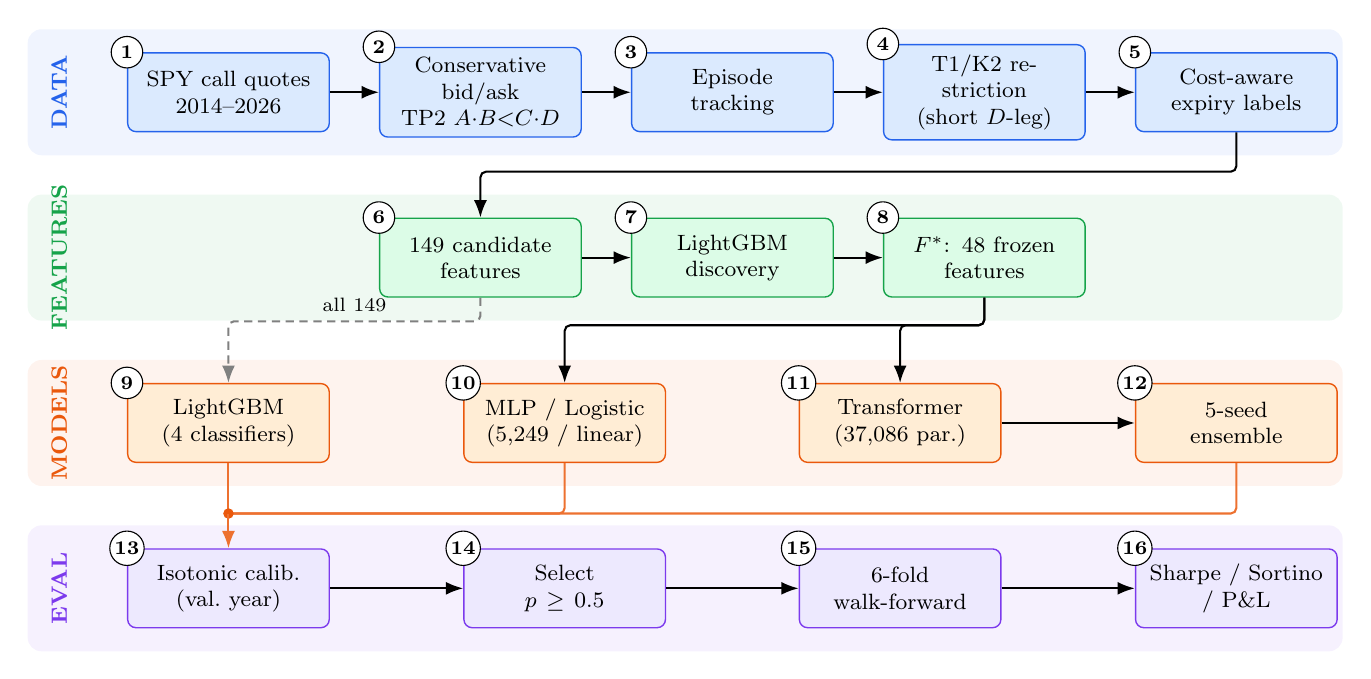
\begin{tikzpicture}[
  every node/.style={font=\footnotesize},
  b/.style={draw, rounded corners=3pt, align=center, text width=2.3cm, minimum height=1.0cm, inner sep=1.3mm, line width=0.5pt},
  bd/.style={b, fill=cData, draw=cDataB}, bf/.style={b, fill=cFeat, draw=cFeatB},
  bm/.style={b, fill=cModel, draw=cModelB}, be/.style={b, fill=cEval, draw=cEvalB},
  arr/.style={-{Latex[length=2.2mm]}, line width=0.75pt, rounded corners=2pt},
  mrg/.style={line width=0.75pt, rounded corners=2pt, cModelB!85},
  brc/.style={-{Latex[length=2.2mm]}, line width=0.75pt, densely dashed, gray, rounded corners=2pt},
  sn/.style={circle, draw, fill=white, font=\scriptsize\bfseries, inner sep=0.3mm, minimum size=4mm}
]
\def\ry{0}\def\rf{-2.1}\def\rm{-4.2}\def\re{-6.3}
\begin{scope}[on background layer]
  \fill[cDataB!7,  rounded corners=5pt] (-2.55,0.80)  rectangle (14.15,-0.80);
  \fill[cFeatB!7,  rounded corners=5pt] (-2.55,-1.30) rectangle (14.15,-2.90);
  \fill[cModelB!7, rounded corners=5pt] (-2.55,-3.40) rectangle (14.15,-5.00);
  \fill[cEvalB!7,  rounded corners=5pt] (-2.55,-5.50) rectangle (14.15,-7.10);
\end{scope}
\node[bd] (n1) at (0,\ry)    {SPY call quotes\\2014--2026};
\node[bd] (n2) at (3.2,\ry)  {Conservative bid/ask\\TP2 $A{\cdot}B{<}C{\cdot}D$};
\node[bd] (n3) at (6.4,\ry)  {Episode\\tracking};
\node[bd] (n4) at (9.6,\ry)  {T1/K2 restriction\\(short $D$-leg)};
\node[bd] (n5) at (12.8,\ry) {Cost-aware\\expiry labels};
\node[bf] (n6) at (3.2,\rf) {149 candidate\\features};
\node[bf] (n7) at (6.4,\rf) {LightGBM\\discovery};
\node[bf] (n8) at (9.6,\rf) {$F^{\ast}$: 48 frozen\\features};
\node[bm] (n9)  at (0,\rm)    {LightGBM\\(4 classifiers)};
\node[bm] (n10) at (4.27,\rm) {MLP / Logistic\\(5{,}249 / linear)};
\node[bm] (n11) at (8.53,\rm) {Transformer\\(37{,}086 par.)};
\node[bm] (n12) at (12.8,\rm) {5-seed\\ensemble};
\node[be] (n13) at (0,\re)    {Isotonic calib.\\(val.\ year)};
\node[be] (n14) at (4.27,\re) {Select\\$p\!\ge\!0.5$};
\node[be] (n15) at (8.53,\re) {6-fold\\walk-forward};
\node[be] (n16) at (12.8,\re) {Sharpe / Sortino\\/ P\&L};
\draw[arr] (n1)--(n2); \draw[arr] (n2)--(n3); \draw[arr] (n3)--(n4); \draw[arr] (n4)--(n5);
\draw[arr] (n5.south) -- ++(0,-0.5) -| (n6.north);
\draw[arr] (n6)--(n7); \draw[arr] (n7)--(n8);
\draw[arr] (n8.south) -- ++(0,-0.35) -| (n11.north);
\draw[arr] (n8.south) -- ++(0,-0.35) -| (n10.north);
\draw[brc] (n6.south) -- ++(0,-0.3) -| (n9.north) node[pos=0.25,above,black,font=\scriptsize]{all 149};
\draw[arr] (n11)--(n12);
\coordinate (jn) at (0,-5.35);
\draw[mrg] (n10.south) |- (jn);
\draw[mrg] (n12.south) |- (jn);
\draw[mrg] (n9.south) -- (jn);
\fill[cModelB] (jn) circle (1.9pt);
\draw[arr, cModelB!85] (jn) -- (n13.north);
\draw[arr] (n13)--(n14); \draw[arr] (n14)--(n15); \draw[arr] (n15)--(n16);
\foreach \n/\l in {n1/1,n2/2,n3/3,n4/4,n5/5,n6/6,n7/7,n8/8,n9/9,n10/10,n11/11,n12/12,n13/13,n14/14,n15/15,n16/16}
  \node[sn] at (\n.north west) {\l};
\node[rotate=90, cDataB,  font=\bfseries\footnotesize] at (-2.15,\ry) {DATA};
\node[rotate=90, cFeatB,  font=\bfseries\footnotesize] at (-2.15,\rf) {FEATURES};
\node[rotate=90, cModelB, font=\bfseries\footnotesize] at (-2.15,\rm) {MODELS};
\node[rotate=90, cEvalB,  font=\bfseries\footnotesize] at (-2.15,\re) {EVAL};
\end{tikzpicture}
}
\caption{Pipeline, steps 1--16. Steps 1--5 build the episode dataset; steps 7--8 select the frozen $F^{\ast}$ dictionary; LightGBM (step 9) trains on all 149 candidates (dashed). All scorers converge on one shared downstream---calibration, $p\ge0.5$ selection, walk-forward evaluation---so the operating-point confound of Section~\ref{sec:confound} arises in the shared stage, not in any model-specific code path.}
\label{fig:pipeline}
\end{figure*}

\medskip\noindent\textbf{Walk-Forward Design.}
We use six rolling folds covering test years 2021--2026: each trains on the three years ending two years before its test year, calibrates (isotonic) on the single intervening validation year, and evaluates once on the test year (so the first fold is 2017--2019 / 2020 / 2021 and the last is 2022--2024 / 2025 / 2026). Feature scaling is fit on training years only and calibration on the validation year only; no test-year information enters either. An expanding-window alternative is evaluated in Section~\ref{sec:robustness}.

\medskip\noindent\textbf{Feature Construction.}
\label{sec:features}
From 149 candidate variables in eight semantic blocks---market, short-leg structure, option risk, surface location, liquidity, TP2 geometry, strategy/calendar, and lifecycle pressure---we construct a fixed 48-feature dictionary $F^{\ast}$ using LightGBM-based~\cite{ke2017lightgbm} importance and temporal-stability criteria. The same feature dictionary is used by all downstream models unless otherwise indicated. Only feature \emph{values} feed the downstream models; LightGBM's predictions and importances are never inputs, so the comparison in Section~\ref{sec:results} is between independent selectors on a shared, inspectable dictionary, not a stacked ensemble. The full feature list and construction procedure are provided with the released implementation.

\noindent\textbf{Implementation (all models).} Every model uses the six folds, training-set standardization, validation-year isotonic calibration, and $p\ge0.5$ selection; single-seed rows use the fixed default seed 42 (set a priori, not best-of-several---though Section~\ref{sec:confound} shows it happens to be the MLP's most favorable seed, which is part of the point), and 5-seed ensembles average raw probabilities over seeds \{42,101,202,303,404\} before one calibration. LightGBM: 350 trees, learning rate 0.04, 31 leaves, min-child 30, sub/colsample 0.8, balanced class weights. MLP (48-64-32-1, ReLU, 5{,}249 parameters): Adam, lr $10^{-3}$, $L_2$ $10^{-4}$, batch 1024, $\le$80 epochs, patience 8. Transformer (37{,}086 parameters): hidden 64, 4 heads, $\le$64 history tokens, AdamW lr $3{\times}10^{-5}$, weight decay $10^{-4}$, 8\% warm-up, grad-clip 1.0, $\le$25 epochs, validation-\emph{loss} checkpointing (an earlier ranking-metric checkpoint allowed calibration-degrading epochs to survive), plus a Huber auxiliary loss on realized return. An $L_2$-regularized logistic regression on $F^{\ast}$ serves as the linear floor.

\medskip\noindent\textbf{The Transformer, Its Distance-Biased Variant, and Ablations.}
\label{sec:transformer}
Each candidate episode-strategy pair is a token combining its $F^{\ast}$ values, a strategy embedding, and calendar features. The token cross-attends to the 64 most recently dated episode tokens from strictly earlier calendar days---selected by date alone, never by label or outcome, zero-padded when fewer exist---with logits
$a^{h}_{ij}=q_i\!\cdot\!k_j/\sqrt{d}\,+\,\text{(same/cross-strategy bonus)}$.

\noindent\textbf{MV-ALiBi variant.} Generalizing ALiBi's scalar penalty~\cite{press2022alibi}, we subtract $m_h^{\top}d_{ij}$ from the logit, where $d_{ij}$ collects five domain distances between episodes $i,j$ (time, surface location, short-leg structure, liquidity, lifecycle stage) and $m_h$ is a softplus-positive learned slope vector (20 extra parameters). The mechanism trains as designed: despite $\sim$7:1 raw scale differences across distances, learned slopes converge to 0.26--0.27 for every distance, head, and seed (30 models). Its \emph{trading} effect, however, is ensembling-dependent: at single seed plain attention wins (Sharpe 1.73 vs.\ 1.51), at five seeds the ranking reverses (2.18 vs.\ 2.36; rows in Table~\ref{tab:consolidated}), and neither gap is significant (two-sided sign tests $p=0.219$ and $p=1.000$; block-bootstrap CIs $[-\$162\text{K},\$405\text{K}]$ and $[-\$135\text{K},\$110\text{K}]$). We evaluate plain attention as primary for simplicity while noting the five-seed evidence favors the variant---a first instance of the confound of Section~\ref{sec:confound}.

\noindent\textbf{No-history and permuted-history ablations.}
\label{sec:ablations}
Removing cross-attention entirely (input projection straight to the head; 16{,}130 parameters) looks decisive at matched single seed---Sharpe 1.73$\to$0.87, positive years 6/6$\to$4/6---but at matched \emph{five-seed} ensembles the gap shrinks to 2.18 vs.\ 1.81 (\$719.9K, 6/6): a real but modest $\approx$0.37, one fifth of the single-seed impression. More telling, a variant keeping all 37{,}086 parameters but attending to 64 \emph{randomly chosen} strictly-earlier episodes reaches 2.14 at five seeds---within 0.04 of the full model. The attention pathway helps; \emph{which} history it attends to barely matters.

\medskip\noindent\textbf{Calibration and Trade Selection.}
\label{sec:calibration}
Isotonic regression~\cite{zadrozny2002transforming} is fit on validation-year predictions and applied unchanged to the subsequent test year. Ensembles average raw seed probabilities before calibration. All models use the same operating rule: an episode-strategy pair is traded when its calibrated probability is at least 0.5. We use a common $p\ge0.5$ operating rule across models and folds.

\section{Results}
\label{sec:results}

All models are evaluated using the same walk-forward folds, validation-year isotonic calibration, and $p\ge0.5$ selection rule, with portfolio metrics computed consistently across all models. We report total normalized P\&L, annualized return-to-variability ratios, win rate, mean trade return, drawdown, and the number of positive test years; detailed metric definitions are provided with the released implementation. Because different models select different numbers and compositions of episode-strategy pairs, fixed-threshold comparisons can conflate predictive quality with selectivity. We therefore supplement them with matched-selectivity curves and capital-constrained portfolio results.

\medskip\noindent\textbf{Unconditional Baseline and the Consolidated Comparison.}
Trading all 250{,}004 eligible episode-strategy pairs (two per episode) over 2021--2026 loses \$12.52M under the \$1{,}000 normalized-exposure convention (active-day Sharpe $-1.01$, max drawdown $-\$24.51$M, win rate 12.9\%, 2/6 positive years). The contrast with the European-style benchmark is the paper's central financial fact. The same four-contract structure wins 95--100\% of the time on SPX at mid-prices~\cite{glasserman2025tp2}. On American-style SPY, detected in executable quotes and charged the spread, it wins 12.9\% of the time. American exercise, discreteness, and transaction costs consume the entire near-arbitrage premium. Each learned selector materially improves on this unconditional baseline, and all four model families produce positive aggregate out-of-sample P\&L (Table~\ref{tab:consolidated}). Two reference rows bracket the result. An $L_2$ logistic regression on $F^{\ast}$ earns \$2.02M (Sharpe 2.27)---above LightGBM and both single-seed deep models---so most of the tradable signal is \emph{linear in the selected features}~\cite{grinsztajn2022why,gorishniy2021revisiting}. Random selection at the MLP's trade count loses \$0.77M (Sharpe $-1.14$), so the gains are not a mechanical consequence of taking fewer trades.

\begin{table}[t]
\centering
\footnotesize
\resizebox{\linewidth}{!}{%
\begin{tabular}{llrrrrrrrr}
\toprule
Method & Seeds & Trades & Total P\&L & Active-day Sharpe & Downside ratio & Win\% & $\bar r$\% & Skew & Pos.\ yrs \\
\midrule
Unconditional & -- & 250{,}004 & $-$\$12.52M & $-$1.01 & $-$2.12 & 12.9 & $-$5.0 & 16.6 & 2/6 \\
LightGBM & 1 & 19{,}636 & \$682K & 1.25 & 1.12 & 50.6 & 3.5 & 9.4 & 5/6 \\
MLP & 1 & 14{,}258 & \$1.41M & 2.60 & 6.89 & 54.0 & 9.9 & 9.6 & 6/6 \\
MLP & 5 & 24{,}977 & \$3.43M & 1.66 & 6.12 & 33.0 & 13.7 & 8.9 & 4/6 \\
Transformer (plain) & 1 & 16{,}435 & \$686K & 1.73 & 1.70 & 57.9 & 4.2 & 1.1 & 6/6 \\
Transformer (plain) & 5 & 14{,}338 & \$695K & 2.18 & 2.98 & 60.0 & 4.8 & 1.8 & 6/6 \\
Transformer (ALiBi) & 1 & 15{,}015 & \$570K & 1.51 & 1.24 & 61.0 & 3.8 & $-$2.3 & 6/6 \\
Transformer (ALiBi) & 5 & 14{,}648 & \$704K & 2.36 & 3.72 & 60.1 & 4.8 & 1.0 & 6/6 \\
\midrule
Logistic (L2) & 1 & 13{,}841 & \$2.02M & 2.27 & 4.20 & 53.5 & 14.6 & 5.5 & 5/6 \\
Random @$N$ & -- & 14{,}258 & $-$\$0.77M & $-$1.14 & -- & -- & -- & -- & -- \\
\bottomrule
\end{tabular}%
}
\caption{All models and seed counts, plus unconditional, linear, and random-at-matched-$N$ baselines, 2021--2026. `Seeds': independently trained models whose raw probabilities are averaged before one calibration. $\bar r$\%: mean per-trade normalized return; dollar figures under the \$1{,}000-per-trade convention. The two most profitable rows (MLP-5, Logistic) also carry the highest right-skew and lowest win rates: their returns are concentrated in relatively infrequent, outsized winners.}
\label{tab:consolidated}
\end{table}

\medskip\noindent\textbf{The Operating-Point Confound.}
\label{sec:confound}
Ensembling acts through two channels at once. It changes the scores---and, because a single isotonic map is refit on the averaged validation probabilities and the threshold stays at $0.5$, it changes \emph{how many trades cross}: $+75\%$ for the MLP (14{,}258$\to$24{,}977), $-13\%$ for the transformer (16{,}435$\to$14{,}338). The two architectures are therefore compared at different points of their own selectivity curves before and after ensembling. Under the fixed-threshold evaluation, the reported ranking reverses (MLP 2.60$\to$1.66; transformer 1.73$\to$2.18). On total P\&L, mean per-trade return, and the capital-scaled backtest of Section~\ref{sec:capitalscaled}, the MLP leads at both seed counts. The reversal is specific to the fixed-threshold, flat-notional evaluation and does not persist across the other portfolio summaries; MLP-5's win rate falls to 33\% while $\bar r$ rises to 13.7\%, so its returns concentrate in fewer, larger winners.

Seed dispersion completes the picture. Across the same five seeds, single-seed MLP Sharpe spans 1.47--2.60 (median 2.07, IQM 2.07)---the 2.60 in Table~\ref{tab:consolidated} is the a-priori default seed 42, which happens to be the most favorable, and the spread exceeds the nominal single-versus-ensemble gap. The transformer is tighter (1.50--1.81, IQM 1.73), and its five-seed ensemble (2.18) beats \emph{every} single seed: ensembling helps the transformer consistently, while the MLP's single-seed point estimate is too noisy to rank architectures on at all.

Formal tests agree that nothing here separates the architectures. Two-sided sign tests on year-by-year P\&L differences: $p=0.688$ single-seed (4/6 years favor MLP), $p=1.000$ five-seed (3--3). A year-level paired bootstrap~\cite{efron1993bootstrap} (20{,}000 resamples) gives a five-seed CI of $[\$18.5\text{K},\$927.1\text{K}]$---excluding zero only because MLP's winning years are far larger---while the trade-dependence-aware block bootstrap~\cite{kunsch1989} (21-day blocks) includes zero at both seed counts (single $[-\$676.5\text{K},\$2.53\text{M}]$; five-seed $[-\$2.16\text{M},\$10.18\text{M}]$); the two tests disagree at five seeds and we report both. With six paired years, sign-test power against a model that truly wins 80\% of years is $\approx$0.26: these nulls are underpowered, not evidence of equivalence~\cite{bouthillier2021accounting,agarwal2021deep}.

\medskip\noindent\textbf{Matched-Selectivity Curves.}
\label{sec:selectivity}
Figure~\ref{fig:selectivity} controls for the operating point directly: sweeping the calibrated threshold over $[0.30,0.85]$ traces Sharpe and Sortino as functions of trade count $N$, so models are compared at \emph{equal selectivity}. Three findings. First, the single-seed MLP dominates both transformer variants at every matched $N$ in the region containing all the $p\ge0.5$ operating points (Sharpe 2.38--2.60 versus 1.63--2.01 for the single transformer and 1.93--2.35 for its five-seed ensemble over $N\approx14$--18K): the MLP-versus-transformer gap of Table~\ref{tab:consolidated} is not an operating-point artifact. Second, within the transformer family the five-seed curve sits above the single-seed curve at every $N$---this ensembling gain is real and selectivity-independent. Third, the MLP's own curve declines from 2.60 toward 2.38--2.45 as $N$ grows from 14K to 18K, quantifying how much of any fixed-threshold comparison is movement \emph{along} a curve rather than \emph{between} models. The one comparison the present sweep cannot adjudicate is five-seed MLP versus five-seed transformer at matched $N$: the ensemble's full-population predictions were not retained by the training script, and we do not assert what that curve would show.
%% TODO-RERUN[67]: when tables/action_list/selectivity_sweep.csv gains the
%% "MLP (5)" rows, replace the final sentence with the matched-N read-off at
%% N ~= 14,338 and update Figure 4 (script regenerates it automatically).
LightGBM's curve uses the sweep's one-action-per-episode convention ($N$ differs $\sim$5\% from its Table~\ref{tab:consolidated} selection file); no comparison here depends on this.

\begin{figure}[t]
\centering
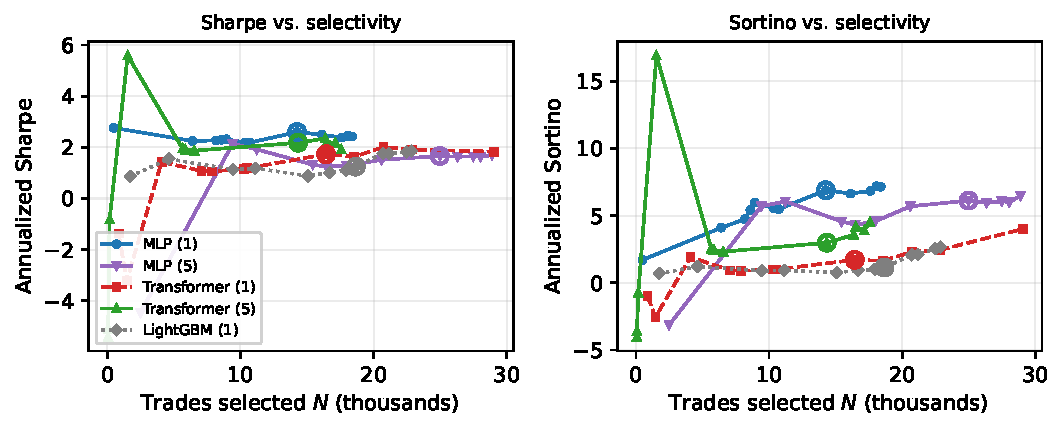
\includegraphics[width=\linewidth]{figures/selectivity_curves.pdf}
\caption{Performance versus selectivity: annualized active-day Sharpe (left) and downside ratio (right) versus the number of trades selected $N$ as the calibrated threshold sweeps 0.30--0.85. Open circles mark $p\ge0.5$ operating points. At matched $N$, the single-seed MLP leads throughout and the five-seed transformer leads its single-seed variant throughout.}
\label{fig:selectivity}
\end{figure}

\medskip\noindent\textbf{Capital-Scaled Backtest: The Deployment Lens.}
\label{sec:capitalscaled}
The \$1{,}000-per-trade convention isolates selection quality but assumes unlimited capital. Under realistic sizing---\$1M starting capital, at most 1\% of available cash committed to new positions each day (the $\kappa=100$ leverage convention of the SPX study~\cite{glasserman2025tp2}), equal weighting within a day, no leverage---the picture changes (Table~\ref{tab:capitalscaled}). LightGBM and the MLP remain profitable. Both transformer variants fall to near-zero CAGR. The cause is payoff shape, not ranking ability: on its lowest-competition days, where per-trade capital is largest, the transformer wins \emph{more} often than LightGBM/MLP (69.9\% vs.\ 59.8\%/54.9\%) with the best discrimination (ROC-AUC 0.906 on this more balanced subset, vs.\ 0.890/0.881), but its wins are small and its losses large (payoff ratio 0.36 versus 4.09/3.54), and its best trades land on its smallest-allocation days. Flat-notional Sharpe overstates what the transformer can capture under a capital constraint. For deployment, the ranking question is settled here: the simpler models win.

\begin{table}[t]
\centering
\footnotesize
\begin{tabular}{lrrrr}
\toprule
Model & CAGR & Sharpe & Max DD & Calmar \\
\midrule
Unconditional & $-11.7\%$ & $-0.67$ & $-70.5\%$ & $-0.17$ \\
LightGBM & 14.6\% & 1.09 & $-6.3\%$ & 2.31 \\
MLP & 17.2\% & 1.03 & $-5.2\%$ & 3.32 \\
Transformer (plain) & 0.6\% & 0.32 & $-3.7\%$ & 0.18 \\
Transformer (ALiBi) & 0.9\% & 0.51 & $-2.5\%$ & 0.37 \\
\bottomrule
\end{tabular}
\caption{Capital-scaled backtest, 2021--2026: \$1M starting capital, 1\%-of-cash daily cap, no leverage. CAGR and drawdown do not depend on the flat-notional convention of Table~\ref{tab:consolidated}.}
\label{tab:capitalscaled}
\end{table}

\medskip\noindent\textbf{Robustness.}
\label{sec:robustness}

\noindent\textbf{Strategy-level breakdown.} At matched single seed (42), K2 is the common profit source: the MLP earns \$1.21M of its \$1.41M on K2 (Sharpe 2.66 vs.\ 1.62 on T1); the single-seed transformer's entire net gain is K2 (\$717K, Sharpe 2.60) against a small T1 loss ($-$\$31K) that turns positive (\$274K) only once ensembled---another ensembling-dependent sign flip; LightGBM is the most balanced (T1 \$378K/0.85, K2 \$304K/1.74). No model's result rests on a single denomination.

\noindent\textbf{Year-by-year.} At matched single seed, unconditional trading loses heavily in four of six test years with swings one to two orders of magnitude larger than any learned model's, while the learned models remain in a narrow, mostly positive band---profitable in different years to different degrees (MLP and transformer 6/6 positive, LightGBM 5/6; Table~\ref{tab:consolidated})---so no conclusion rests on a single model or year.

\noindent\textbf{Excluding the partial year.} 2026 covers $\approx$107 trading days; re-running on 2021--2025 leaves every conclusion intact (MLP-1 \$1.38M/2.59; five-seed transformer \$532K/1.92) and \emph{strengthens} the baseline contrast: unconditional worsens to $-\$17.45$M (Sharpe $-1.73$, 1/5 positive years).

\noindent\textbf{Training window.} An expanding window earns more raw dollars (\$734.9K vs.\ \$686.2K) from higher late-sample volume at lower quality, but loses on Sharpe in five of six years with the only negative year (2024, $-0.13$ vs.\ 1.59); we keep the three-year window.

\noindent\textbf{Execution and early assignment.} At $1.5\times$ quoted-spread slippage, all rankings and positive-year counts are unchanged; Sharpe falls 7\% (transformers) to 37\% (LightGBM). Trades whose short leg spans an ex-dividend date (early-assignment risk the expiry labels do not price) are 16--22\% of selections; LightGBM's exposed subset is net negative ($-\$33$K) while the transformer's has a \emph{higher} win rate than its unexposed one---reported without a causal account.

\noindent\textbf{Market exposure.} Regressing each trade's realized return on the underlying's return over the corresponding holding window, which averages 3.6 days, shows a statistically significant positive exposure for all three models (MLP $\beta=7.2$, $t=11.5$; transformer $0.9$; LightGBM $0.7$; all $R^2<0.006$). The low $R^2$ makes the tilt noisy, not small: for the MLP, a $+1\%$ underlying move over a typical hold shifts expected trade return by $+7.2$ percentage points---roughly half its 13.7\% mean per-trade return---over a strongly rising 2021--2026 market. These strategies are long-biased, not market-neutral. Reconciling the positive realized beta with predominantly net-short entry delta (75--82\% of trades, a structural consequence of shorting the near leg) requires path-dependent effects we have not isolated, and we flag the tension openly. Separately, sensitivity to an average-IV proxy (we did not merge external VIX data) is small but significant for the transformer variants only ($r\approx0.10$, $p<0.005$). Against the \emph{unconditional} baseline, the block bootstrap finds the Sharpe improvement significant for the MLP and both transformer variants but not LightGBM (CI $[-0.03,4.13]$).

\noindent\textbf{Classification metrics.} On the pooled test population (base rate $\approx$13.8\%, identical across models by construction), Table~\ref{tab:calibration} shows no model dominating: LightGBM discriminates best (PR-AUC 0.492) despite the weakest P\&L among learned models; the plain transformer calibrates best (ECE 0.024). ROC-AUC is base-rate-invariant; we report PR-AUC because it is the more informative summary for a rare positive class, and ROC-AUC only on the balanced quiet-day subset above. The five-seed no-history ablation's PR-AUC (0.451) trails both transformer variants---seed-matched evidence that attention adds discrimination, consistent with its modest trading gain.

\begin{table}[t]
\centering
\footnotesize
\begin{tabular}{lrrr}
\toprule
Model & PR-AUC & Brier & ECE \\
\midrule
LightGBM & 0.492 & 0.086 & 0.049 \\
MLP & 0.406 & 0.096 & 0.036 \\
Transformer (plain, 5-seed) & 0.458 & 0.083 & 0.024 \\
Transformer (ALiBi, 5-seed) & 0.460 & 0.083 & 0.028 \\
No-history ablation (5-seed) & 0.451 & 0.089 & 0.046 \\
\bottomrule
\end{tabular}
\caption{PR-AUC (average precision), Brier score, and expected calibration error (10 equal-width bins) on the pooled 2021--2026 test population (base rate $\approx$13.8\%).}
\label{tab:calibration}
\end{table}

\section{Discussion and Threats to Validity}
\label{sec:limitations}

\noindent\textbf{What this adds to the TP2 literature.} The theory says when prices should be TP2~\cite{glasserman2026tp2theory}. The SPX study shows that mid-price violations on a European-style, cash-settled index are near-arbitrage~\cite{glasserman2025tp2}. Our results locate the boundary of that finding. Moving to American-style, dividend-paying SPY and to executable quotes does not make violations disappear; 177{,}487 episodes survive the stricter screen. It does invert their unconditional economics: a 12.9\% win rate instead of 95--100\%. The violation premium of Equation~\eqref{eq:tp2adj} is still collected at entry. On American calls, however, it no longer covers the short leg's assignment and dividend risk plus the spread, except in a subset of episodes. That subset can be identified from TP2 geometry, surface location, short-leg structure, liquidity, and lifecycle features, by any calibrated classifier including a linear one. This is the financial contribution: under frictions, the TP2 restriction still contains tradable relative-value information outside the setting where it is provable.

\noindent\textbf{What carries the signal.} A linear model on $F^{\ast}$ matches or beats every deep configuration except the single-seed MLP's most favorable draw. Permuting the attended history costs 0.04 Sharpe. Only the transformer family shows IV-proxy sensitivity and the capital-scaled decline. The conclusion is that the episode construction and the feature dictionary carry the signal. On this evidence, architecture choices beyond a calibrated classifier, even a linear one, are second-order. This matches the tabular-data literature~\cite{grinsztajn2022why,gorishniy2021revisiting}.

\noindent\textbf{Validity.} The known threats, in decreasing order of concern: (i) the $\sim$4$\times$ base-rate shift between the early training folds and all test years, absorbed only by a one-year isotonic fit, with fold-level performance tracking the mismatch; (ii) no scale-invariant, moneyness-style price-ratio feature in $F^{\ast}$ while the underlying drifts 50--80\% across the sample; (iii) TP2 is proved for European cash-settled index options, not American SPY calls~\cite{glasserman2026tp2theory,cosma2020earlyexercise}---we treat it as an empirical hypothesis, with 16--22\% of selected trades carrying short-leg ex-dividend timing; (iv) no vertical/calendar no-arbitrage pre-filter, reported elsewhere to matter little~\cite{glasserman2025tp2}. All code and derived episode/feature/label datasets will be released on acceptance; the raw vendor quote feed cannot be redistributed.

\section{Conclusion}
Violations of the TP2 restriction are near-arbitrage on European-style index options at mid-prices~\cite{glasserman2025tp2,glasserman2026tp2theory}. On American-style SPY calls, detected in executable quotes and charged realistic costs, trading them unconditionally loses money. The signal remains tradable conditionally. Learned selectors on 48 TP2-aware features turn a \$12.52M unconditional loss into positive out-of-sample returns under the same causal $p\ge0.5$ selection rule. The result survives slippage stress, early-assignment accounting, and capital-constrained sizing at the SPX study's convention. This locates the economic boundary of the TP2 near-arbitrage, and shows that crossing it is a selection problem that can be learned, not a detection problem. On methodology: comparing the selectors exposed an operating-point confound. The decision rule ties the portfolio to the model, so ensembling moved trade counts by $+75\%$ and $-13\%$ and reversed flat-notional Sharpe rankings. Matched-selectivity curves and seed-dispersion intervals show that the apparent rankings are sensitive to model operating points and random initialization: no architecture wins, the feature construction carries the signal, and under deployment-relevant sizing the simplest models lead. Open problems: a scale-invariant feature dictionary, early-exercise-aware labels for the short leg, completing the supermodular route to American TP2, and reconciling the positive realized beta with short entry delta.

\bibliographystyle{ACM-Reference-Format}
\begingroup
\footnotesize
\setlength{\itemsep}{0pt}
\setlength{\parskip}{0pt}
\begin{thebibliography}{27}

\bibitem{glasserman2025tp2}
Paul Glasserman, Mike Li, and Dan Pirjol. 2025. Trading TP\textsubscript{2} Option Violations. Working paper, SSRN 5392317. July 2025.

\bibitem{press2022alibi}
Ofir Press, Noah A. Smith, and Mike Lewis. 2022. Train Short, Test Long: Attention with Linear Biases Enables Input Length Extrapolation. In \textit{International Conference on Learning Representations (ICLR)}.

\bibitem{glasserman2026tp2theory}
Paul Glasserman and Dan Pirjol. 2026. When Are Option Prices TP\textsubscript{2}? \textit{Mathematical Finance} 36, 3 (2026). \url{https://doi.org/10.1111/mafi.70024}

\bibitem{glasserman2023convexity}
Paul Glasserman and Dan Pirjol. 2023. Total Positivity and Relative Convexity of Option Prices. \textit{Frontiers of Mathematical Finance} 2, 1 (2023), 1--32.

\bibitem{merton1973}
Robert C. Merton. 1973. Theory of Rational Option Pricing. \textit{Bell Journal of Economics and Management Science} 4, 1 (1973), 141--183.

\bibitem{black1975}
Fischer Black. 1975. Fact and Fantasy in the Use of Options. \textit{Financial Analysts Journal} 31, 4 (1975), 36--41, 61--72.

\bibitem{topkis1998}
Donald M. Topkis. 1998. \textit{Supermodularity and Complementarity}. Princeton University Press.

\bibitem{vershynin2026}
Roman Vershynin. 2026. \textit{High-Dimensional Probability} (2nd ed.). Cambridge University Press.

\bibitem{ke2017lightgbm}
Guolin Ke et al. 2017. LightGBM: A Highly Efficient Gradient Boosting Decision Tree. In \textit{NeurIPS 30}.

\bibitem{zadrozny2002transforming}
Bianca Zadrozny and Charles Elkan. 2002. Transforming Classifier Scores into Accurate Multiclass Probability Estimates. In \textit{KDD}.

\bibitem{cosma2020earlyexercise}
Antonio Cosma et al. 2020. Early Exercise Decision in American Options with Dividends, Stochastic Volatility, and Jumps. \textit{J.\ Financial and Quantitative Analysis} 55, 1 (2020), 331--356.

\bibitem{kearns2013mlmicrostructure}
Michael Kearns and Yuriy Nevmyvaka. 2013. Machine Learning for Market Microstructure and High Frequency Trading. In \textit{High-Frequency Trading}. Risk Books.

\bibitem{efron1993bootstrap}
Bradley Efron and Robert J. Tibshirani. 1993. \textit{An Introduction to the Bootstrap}. Chapman \& Hall.

\bibitem{kunsch1989}
Hans R. K\"unsch. 1989. The Jackknife and the Bootstrap for General Stationary Observations. \textit{Annals of Statistics} 17, 3 (1989), 1217--1241.

\bibitem{bailey2014deflated}
David H. Bailey and Marcos L\'opez de Prado. 2014. The Deflated Sharpe Ratio: Correcting for Selection Bias, Backtest Overfitting, and Non-Normality. \textit{Journal of Portfolio Management} 40, 5 (2014), 94--107.

\bibitem{harvey2016crosssection}
Campbell R. Harvey, Yan Liu, and Heqing Zhu. 2016. $\ldots$ and the Cross-Section of Expected Returns. \textit{Rev.\ Financial Studies} 29, 1 (2016), 5--68.

\bibitem{white2000reality}
Halbert White. 2000. A Reality Check for Data Snooping. \textit{Econometrica} 68, 5 (2000), 1097--1126.

\bibitem{bouthillier2021accounting}
Xavier Bouthillier et al. 2021. Accounting for Variance in Machine Learning Benchmarks. In \textit{MLSys} 3.

\bibitem{dodge2019show}
Jesse Dodge et al. 2019. Show Your Work: Improved Reporting of Experimental Results. In \textit{EMNLP-IJCNLP}.

\bibitem{melis2018state}
G\'abor Melis, Chris Dyer, and Phil Blunsom. 2018. On the State of the Art of Evaluation in Neural Language Models. In \textit{International Conference on Learning Representations (ICLR)}.

\bibitem{lucic2018gans}
Mario Lucic et al. 2018. Are GANs Created Equal? A Large-Scale Study. In \textit{NeurIPS 31}.

\bibitem{agarwal2021deep}
Rishabh Agarwal et al. 2021. Deep Reinforcement Learning at the Edge of the Statistical Precipice. In \textit{NeurIPS 34}.

\bibitem{grinsztajn2022why}
L\'eo Grinsztajn, Edouard Oyallon, and Ga\"el Varoquaux. 2022. Why Do Tree-Based Models Still Outperform Deep Learning on Typical Tabular Data? In \textit{NeurIPS 35 D\&B}.

\bibitem{gorishniy2021revisiting}
Yury Gorishniy et al. 2021. Revisiting Deep Learning Models for Tabular Data. In \textit{NeurIPS 34}.

\bibitem{shaw2018self}
Peter Shaw, Jakob Uszkoreit, and Ashish Vaswani. 2018. Self-Attention with Relative Position Representations. In \textit{NAACL-HLT}.

\bibitem{bali2023option}
Turan G. Bali et al. 2023. Option Return Predictability with Machine Learning and Big Data. \textit{Rev.\ Financial Studies} 36, 9 (2023), 3548--3602.

\end{thebibliography}
\endgroup

\end{document}
